
\documentclass[11pt]{beamer}
\usetheme{Copenhagen}
\usecolortheme{wolverine}
\usepackage{multirow}
\usepackage{pifont}
\usepackage{bm}
\usepackage{caption}
\usepackage{subcaption}
\usepackage{url}

\setbeamertemplate{footline}[frame number]
\setbeamertemplate{itemize items}[triangle]
\setbeamertemplate{frametitle}[default][center]




%%% ========================================================
%% For the cover page
%% ========================================================
% la ligne ci-dessous est à insérer obligatoirement dans le préambule du document avant \begin{document}
\usepackage[a4paper]{./cover/meta-donnees} % for the title page

%% ========================================================
%% General packages
%% ========================================================

\usepackage{times,amsmath,amssymb,amsfonts,color,graphicx,latexsym,amsthm}
% \usepackage{xcolor}
\usepackage[table,dvipsnames]{xcolor}
\usepackage{booktabs} % for better tables

\usepackage{tikz,array}
\usetikzlibrary{arrows,automata,calc,decorations.pathmorphing, backgrounds,fit, shapes}

\usepackage{amsmath}
\usepackage{amssymb}
\usepackage{algorithm, algpseudocode}
\usepackage{setspace} % used with \begin{spacing}{..}..\end{spacing}  --> needed in book
% 
\usepackage[normalem]{ulem}

\usepackage{datetime}

\graphicspath{ {figures/} }
% \usepackage{caption}
\usepackage[font={small}]{caption}
\usepackage{subcaption}
% \usepackage[labelformat=simple]{subcaption}
% \renewcommand\thesubfigure{(\alph{subfigure})}  % subfigure with parenthesis, e.g., Figure 1.2(a)
% \renewcommand\thesubfigure{-\alph{subfigure}}   % subfigure with dash, e.g., Figure 1.2-a
\usepackage{multirow}
% \captionsetup{justification=centering}
% \usepackage[caption=true]{subfig}

\usepackage{enumitem} % to change list styling globally

%% ========================================================
% % for the geometry of the pages
%% ========================================================
% \setlength{\parindent}{3.0em}
% \setlength{\parskip}{0.5em}
% \linespread{1.1}  % space between lines
% \usepackage{fullpage}  % decrease margins
% \usepackage{a4wide}
% \usepackage{showframe}   % shows the frames of the pages

%% ========================================================
% Set depth of TOC
%% ========================================================
% \setcounter{tocdepth}{2}
% \settocdepth{subsection}
% \setsecnumdepth{subsection}

%% ========================================================
%% for the mini-toc - have a toc in the beginning of each chapter
%% ========================================================
% \usepackage{minitoc}
% \setcounter{minitocdepth}{1} 
%\nomtcrule       % removes rules = horizontal lines
%\nomtcpagenumbers  % remove page numbers from minitocs
% \dominitoc %% \dominitoc[n] removes contents, \dominitoc[c] centers contents


%% ========================================================
% % %% Make an index list
%% ========================================================
% % \usepackage{imakeidx}
% % \makeindex[title=Index, options= -s ./stylefiles/myIndexStyle.ist, intoc, columns=1]


%% ========================================================
%%%% Style of Chapters 
%% ========================================================

% \usepackage[Lenny]{fncychap}
% \usepackage[Sonny]{fncychap}
% \usepackage[Rejne]{fncychap}
% \usepackage[Bjarne]{fncychap}
% \usepackage[Bjornstrup]{fncychap}
% \usepackage[Conny]{fncychap} %%  incompatible with toc


%% My STYLE
%% Set introduction chapter to 0
% \setcounter{chapter}{-1}

%% My STYLE 
\usepackage{fancyhdr}
\addtolength{\headheight}{\baselineskip}
\fancyhead{} % clear all header fields
\fancyhead[RE]{\leftmark}
\fancyhead[LO]{\rightmark}
\fancyhead[LE,RO]{\thepage}
\fancyfoot{} % clear all footer fields
\fancyfoot[RO,LE]{\textcolor{gray}{\today\ (\currenttime)}}

\usepackage{titlesec}
% % % % % \titleformat{command}[shape]{format}{label}{sep}{before}[after]
% % % % % \titlespacing{<command>}{<left>}{<before-sep>}{<after-sep>}[<right>]

%%%%%%%%%%%%%%%%%%%%%%%%%%%%%%%%%%%%%%%%%%%%%%%%%%%%%%%%%%%%%%%%%%%
%%%%% % Simple Chapter title aligned right
% \titleformat{\chapter}[display]{\color{black}\normalfont\LARGE\bfseries\raggedleft}{\chaptertitlename\ \thechapter}{20pt}{\Huge}

%%%%%%%%%%%%%%%%%%%%%%%%%%%%%%%%%%%%%%%%%%%%%%%%%%%%%%%%%%%%%%%%%%%
%%%%% white Chapter number on black box
% \titleformat{\chapter}[display]{\color{black}\normalfont\LARGE\bfseries\raggedleft}{\textsc{\chaptertitlename}\ \marginpar{\fontsize{50}{60}\selectfont\textcolor{white}{\colorbox{black!50}{\makebox(64,64)\thechapter}}}}{20pt}{\Huge}

%%%%%%%%%%%%%%%%%%%%%%%%%%%%%%%%%%%%%%%%%%%%%%%%%%%%%%%%%%%%%%%%%%%
%%% calligraphic Chapter number in the margin (aurical)
% \usepackage{aurical}
% \usepackage[T1]{fontenc}
% \titleformat{\chapter}[display]{\color{black}\normalfont\LARGE\bfseries\raggedleft}{\textsc{\chaptertitlename}\ \marginpar{\hspace{-1em}\Fontauri\fontsize{100}{120}\selectfont\textcolor{black!30}{\thechapter}}}{20pt}{\Huge}

%%%%% calligraphic Chapter number in the margin (humanist)
% \usepackage{humanist}
% \usepackage[T1]{fontenc}
% \titleformat{\chapter}[display]{\color{black}\normalfont\LARGE\bfseries\raggedleft}{\textsc{\chaptertitlename}\ \marginpar{\hminfamily \fontsize{100}{120}\selectfont\textcolor{black!30}{\thechapter}}}{20pt}{\Huge}

% %%%%%% calligraphic Chapter number in the margin (square caps)
% \usepackage{sqrcaps}
% \usepackage[T1]{fontenc}
% \titleformat{\chapter}[display]{\color{black}\normalfont\LARGE\bfseries\raggedleft}{\textsc{\chaptertitlename}\ \marginpar{\sqrcfamily \fontsize{75}{90}\selectfont\textcolor{black!40}{\colorbox{black!10}{\mbox{\thechapter}}}}}{20pt}{\Huge}

%%%%%%%%%%%%%%%%%%%%%%%%%%%%%%%%%%%%%%%%%%%%%%%%%%%%%%%%%%%%%%%%%%%
%%%%% %%% Big Gray Chapter number in the margin
% \titleformat{\chapter}[display]{\color{black}\normalfont\LARGE\bfseries\raggedleft}{\textsc{\chaptertitlename}\ \marginpar{\fontsize{100}{120}\selectfont\textcolor{black!30}{\thechapter}}}{20pt}{\Huge}

%%%%%%%%%%%%%%%%%%%%%%%%%%%%%%%%%%%%%%%%%%%%%%%%%%%%%%%%%%%%%%%%%%%
%%%%% %% white Chapter number on gray box in the margin - with vertical ``chapter''
% \titleformat{\chapter}[display]{\color{black}\normalfont\LARGE\bfseries\raggedleft}{\rotatebox{90}{\textsc{\chaptertitlename}}\ \marginpar{\hspace{-.7em}\fontsize{60}{72}\selectfont\textcolor{white}{\colorbox{black!50}{\makebox(64,80)\thechapter}}}}{.5em}{\Huge}

% %% white Chapter number on gray box - with vertical ``chapter''
% \titleformat{\chapter}[display]{\color{black}\normalfont\LARGE\bfseries\raggedleft}{\rotatebox{90}{\textsc{\chaptertitlename}}\ {\fontsize{60}{72}\selectfont\textcolor{white}{\colorbox{black!50}{\makebox(64,80)\thechapter}}}}{.5em}{\Huge}

% %% white Chapter number on black box inline- with vertical ``chapter''
\titleformat{\chapter}[display]{\color{black}\normalfont\LARGE\bfseries\raggedleft}{\rotatebox{90}{\textsc{\chaptertitlename}}\ {\hspace{0em}\fontsize{60}{72}\selectfont\textcolor{black!80}{\colorbox{red!20!black!10}{\makebox(64,80)\thechapter}}}}{.5em}{\Huge}


%% ========================================================
%%% Add background to all figures
%% ========================================================
% 
% \usepackage{mdframed}
% 
% \let\originalfigure=\figure
% \let\endoriginalfigure=\endfigure
% 
% \renewenvironment{figure}[1][]{
%   \begin{originalfigure}[#1]
%     \begin{mdframed}[linecolor=black!5,backgroundcolor=black!5]
% }{
%     \end{mdframed}
%   \end{originalfigure}
% }

%% ========================================================
%% Hyperef
%% ========================================================

\usepackage[pagebackref=true]{hyperref} % load hyperref last 
\hypersetup{linktocpage,linktoc=all}
\hypersetup{colorlinks=true,linkcolor=blue,urlcolor=blue,citecolor=blue,filecolor=blue}

% for adding backreference in the bibliography
\renewcommand*{\backref}[1]{}
\renewcommand*{\backrefalt}[4]{({\it%
    \ifcase #1 Not cited.%
          \or Cited on page~#2.%
          \else Cited on pages #2.%
    \fi%
    })}

% Symbols
\newcommand{\ra}{\rightarrow}
\newcommand{\ov}{\overline}
\newcommand{\ur}{\underline}
\newcommand{\pr}{\prime}
\newcommand{\tbf}{\textbf}
\newcommand{\omg}{\Omega}
\newcommand{\mc}{\mathcal}
\newcommand{\lt}{\left}
\newcommand{\rt}{\right}
\newcommand{\mb}{\mathbb}
\newcommand{\imp}{\implies}
\newcommand{\dimp}{\Leftrightarrow}
\newcommand{\wh}{\widehat}
\newcommand{\dg}{\mc{D}}


% Sets
\newcommand{\realset}{\mb{R}}
\newcommand{\comprealset}{\mb{\ov{R}}}
\newcommand{\pint}{\mb{Z}_{> 0}}
\newcommand{\wholenums}{\mb{Z}_\geq 0}
\newcommand{\nzrl}{\mb{R}_{\geq 0}}
\newcommand{\prl}{\mb{R}_{>0}}
\newcommand{\rl}{\mb{R}}
\newcommand{\fin}{\forall i\in\{1,...,n\}}
\newcommand{\tup}[1]{\{1,...,#1\}}
\newcommand{\seq}[2]{_{#1=1}^#2}
\newcommand{\mCnn}{\mb{M}_{n\times n}(\mb{C})}
\newcommand{\mCmm}{\mb{M}_{m\times m}(\mb{C})}
\newcommand{\mCpn}{\mb{M}_{p\times n}(\mb{C})}
\newcommand{\mCnm}{\mb{M}_{n\times m}(\mb{C})}
\newcommand{\mRnn}{\mb{M}_{n\times n}(\mb{R})}
\newcommand{\mRpn}{\mb{M}_{p\times n}(\mb{R})}
\newcommand{\mRnm}{\mb{M}_{n\times m}(\mb{R})}
\newcommand{\mRno}{{{\mb{R}}}^n_{\geq 0}}
\newcommand{\mRmo}{{{\mb{R}}}^m_{\geq 0}}
\newcommand{\mRo}{\mb{R}_{\geq 0}}
\newcommand{\mRn}{{\mb{R}}^n}
\newcommand{\mRm}{{\mb{R}}^m}
\newcommand{\mCn}{\mb{C}^n}
\newcommand{\mCm}{\mb{C}^m}
\newcommand{\inv}{\mb{GL}_n(\mb{R})}
\newcommand{\id}[1]{\mb{I}_{#1\times #1}}
\newcommand{\mat}[3]{\mb{M}_{#1\times #2}(\mb{#3})}


% matrix operations
\newcommand{\ColumnJoin}[2]{\left[\begin{array}{l}{#1}\\{#2} \end{array}\right]}
\newcommand{\cjoin}[3]{\begin{array}{l}#1\\#2\\#3\end{array}}
\newcommand{\pseudoinverse}[1]{#1^\dagger}
\newcommand{\pinv}{\pseudoinverse}

%% Local macros:

% Operators
\DeclareMathOperator{\real}{\operatorname{Re}}
\newcommand{\minaffine}[2]{\widehat{\Lambda}\lt(#1,#2\rt)}
\newcommand{\maxaffine}[2]{\overline{\Lambda}\lt(#1,#2\rt)}
\newcommand{\minaffinefunc}{\widehat{\Lambda}}
\newcommand{\maxaffinefunc}{\overline{\Lambda}}
\newcommand{\minaffineset}{\widehat{\Delta}}
\newcommand{\maxaffineset}{\overline{\Delta}}

% Set notations
\newcommand{\zon}[3]{\mathcal{Z}\lt(#1,#2,#3\rt)}
\newcommand{\CZ}{\lt(V,c,s\rt)}
\newcommand{\GCZ}{\gcz{V}{c}{s}{W}{l}{u}}
\newcommand{\cz}[3]{\mc{C}\lt(#1,#2,#3\rt)}
\newcommand{\CZO}{\lt(V,0,s\rt)}
\newcommand{\czo}[2]{\mc{Z}\lt(#1,0,#2\rt)}
\newcommand{\trj}[2]{{\bf #1}(#2)}
\newcommand{\IncTcz}[6]{\mc{T}\lt(#1,#2,#3,#4,#5,#6\rt)}
\newcommand{\IncGcz}[6]{\mc{G}\lt(#1,#2,#3,#4,#5,#6\rt)}
\newcommand{\Ptope}[3]{\mc{P}\left(#1,#2,#3\right)}
\newcommand{\gcz}[6]{\mathcal{G}\lt(#1,#2,#3,#4,#5,#6\rt)}
\newcommand{\sptope}[3]{\mathcal{P}\lt(#1,#2,#3\rt)}
\newcommand{\scalebound}[5]{\max_{i=1}^{#4}\lt(\lt(\sum_{j=1}^{#5}\lt|#1\rt|_j\rt)-#3_i+#2_i\rt)}
\newcommand{\contemp}[1]{#1^T\lt(#1#1^T\rt)^{-1}}
\newcommand{\sectemp}[1]{\contemp{\ptemplate\lt(#1\rt)}}

% System notations
\newcommand{\system}{\mb{H}}
\newcommand{\locationset}{Q}
\newcommand{\edgeset}{E}
\newcommand{\stay}{\gamma}
\newcommand{\linearmapset}{\mc{A}}
\newcommand{\inputset}{U}
\newcommand{\initialset}{\Omega}
\newcommand{\edge}{\sigma}
\newcommand{\loc}{q}
\newcommand{\map}{\linearmapset}
\newcommand{\inp}{\inputset}
\newcommand{\ptemplate}{\mc{K}}
\newcommand{\systrj}[2]{\lt({\bf #1},{\bf #2}\rt)}
\newcommand{\preloc}[1]{#1_{1}}
\newcommand{\postloc}[1]{#1_{2}}
\newcommand{\upperedgebound}[1]{#1^+}
\newcommand{\loweredgebound}[1]{#1^-}
\newcommand{\reset}[1]{#1_r}
\newcommand{\locationtransition}[1]{R_{#1}}
\newcommand{\edgetransition}[1]{R_{#1}}
\newcommand{\staysptope}[1]{\sptope{\ptemplate\lt(#1\rt)}{\stay^-\lt(#1\rt)}{\stay^+\lt(#1\rt)}}
\newcommand{\guardsptope}[1]{\sptope{\ptemplate\lt(\preloc{#1}\rt)}{\max\lt(\loweredgebound{#1},\stay^-\lt(\preloc{#1}\rt)\rt)}{\min\lt(\upperedgebound{#1},\stay^+\lt(\preloc{#1}\rt) \rt)}}
\newcommand{\hybridset}{\Gamma}

% Equations
\newcommand{\transfer}[4]{#1#4 = #2\dg\lt(#3\rt)}
\newcommand{\centertransfer}[4]{#1#4 = #3-#2}



\newcommand{\mb}{\mathbb}
\newcommand{\mCnn}{\mb{M}_{n\times n}(\mb{C})}
\newcommand{\mCmm}{\mb{M}_{m\times m}(\mb{C})}
\newcommand{\mCpn}{\mb{M}_{p\times n}(\mb{C})}
\newcommand{\mCnm}{\mb{M}_{n\times m}(\mb{C})}
\newcommand{\mRnn}{\mb{M}_{n\times n}(\mb{R})}
\newcommand{\mRpn}{\mb{M}_{p\times n}(\mb{R})}
\newcommand{\mRnm}{\mb{M}_{n\times m}(\mb{R})}
\newcommand{\mRno}{{{\mb{R}}}^n_{\geq 0}}
\newcommand{\omRno}{{\ov{\mb{R}}}^n_{\geq 0}}
\newcommand{\mRmo}{{{\mb{R}}}^m_{\geq 0}}
\newcommand{\omRmo}{{\ov{\mb{R}}}^m_{\geq 0}}
\newcommand{\mRo}{\mb{R}_{\geq 0}}
\newcommand{\omRo}{\ov{\mb{R}}_{\geq 0}}
\newcommand{\mRn}{{\mb{R}}^n}
\newcommand{\omRp}{{\ov{\mb{R}}}^p}
\newcommand{\mRm}{{\mb{R}}^m}
\newcommand{\omRm}{\ov{\mb{R}}^m}
\newcommand{\mCn}{\mb{C}^n}
\newcommand{\mCm}{\mb{C}^m}

% eigenvectors
\newcommand{\eigenvectors}{\Xi}
% contraction in neighborhood
\newcommand{\cont}[3]{\eta_{#1}^{#2}\lt(#3\rt)}


\definecolor{magenta(dye)}{rgb}{0.79, 0.08, 0.48}
\definecolor{calpolypomonagreen}{rgb}{0.12, 0.3, 0.17}
\definecolor{coolblack}{rgb}{0.0, 0.18, 0.39}
\definecolor{palatinatepurple}{rgb}{0.41, 0.16, 0.38}
\definecolor{pansypurple}{rgb}{0.47, 0.09, 0.29}
\definecolor{prune}{rgb}{0.44, 0.11, 0.11}
\definecolor{outrageousorange}{rgb}{1.0, 0.43, 0.29}
\definecolor{mediumjunglegreen}{rgb}{0.11, 0.21, 0.18}
\definecolor{lincolngreen}{rgb}{0.11, 0.35, 0.02}
\definecolor{forestgreen(traditional)}{rgb}{0.0, 0.27, 0.13}
\definecolor{darksienna}{rgb}{0.24, 0.08, 0.08}
\definecolor{carminepink}{rgb}{0.92, 0.3, 0.26}
\definecolor{byzantium}{rgb}{0.44, 0.16, 0.39}
\definecolor{aureolin}{rgb}{0.99, 0.93, 0.0}
\definecolor{carrotorange}{rgb}{0.93, 0.57, 0.13}
\definecolor{daffodil}{rgb}{1.0, 1.0, 0.19}
\definecolor{darklava}{rgb}{0.28, 0.24, 0.2}
\definecolor{caputmortuum}{rgb}{0.35, 0.15, 0.13}
\definecolor{bulgarianrose}{rgb}{0.28, 0.02, 0.03}
\definecolor{armygreen}{rgb}{0.29, 0.33, 0.13}
\definecolor{darkmidnightblue}{rgb}{0.0, 0.2, 0.4}
\definecolor{darkjunglegreen}{rgb}{0.1, 0.14, 0.13}
\definecolor{darkgreen}{rgb}{0.0, 0.2, 0.13}
\definecolor{darkscarlet}{rgb}{0.34, 0.01, 0.1}
\definecolor{darkslategray}{rgb}{0.18, 0.31, 0.31}
\definecolor{darkorchid}{rgb}{0.6, 0.2, 0.8}
\definecolor{darkmidnightblue}{rgb}{0.0, 0.2, 0.4}
\definecolor{darkblue}{rgb}{0.0, 0.0, 0.55}
\definecolor{sealbrown}{rgb}{0.2, 0.08, 0.08}
\definecolor{onyx}{rgb}{0.06, 0.06, 0.06}
\definecolor{neonfuchsia}{rgb}{1.0, 0.25, 0.39}
\definecolor{indianred}{rgb}{0.8, 0.36, 0.36}
\definecolor{darkred}{rgb}{0.55, 0.0, 0.0}
\definecolor{carmine}{rgb}{0.59, 0.0, 0.09}
\definecolor{cosmiclatte}{rgb}{1.0, 0.97, 0.91}
\definecolor{snow}{rgb}{1.0, 0.98, 0.98}



\input{titlepage}

%\setbeamercolor{title}{bg=snow}
%\setbeamercolor{title}{fg=darkblue}
\title{A Calculus of Complex Zonotopes for \\ Invariant and Stability Verification \\of Affine Hybrid Systems}
\setbeamercolor{author}{fg=darkblue}
\author[shortname]{ {\Large  Arvind\ Adimoolam}\vspace{-2em}}
%\setbeamercolor{institute}{fg=calpolypomonagreen}
%% \institute{
%% \center
%% \includegraphics[scale=0.15]{figures/LogoVERIMAG.png}
%% VERIMAG \includegraphics[scale=0.03]{logo-uga-vo-cmjn.jpg}
%% }


\date{}

\begin{document}

% Title page
\begin{frame}[plain]
\maketitle
%
%
\begin{minipage}{1\textwidth}
\vspace{-4em}
\begin{minipage}{0.3\textwidth}
{\footnotesize {\it Reviewers}}\\
{\small Sylvie Putot\\
Mahesh Viswanathan}
\end{minipage}
%
\hspace{2em}
\begin{minipage}{0.3\textwidth}
{\footnotesize {\it Supervised by}}\\
{\small Thao Dang}
\end{minipage}
%
\begin{minipage}{0.25\textwidth}
{\footnotesize {\it Examiners}}\\
{\small Laurent Fribourg\\
Luc Jaulin}
\end{minipage}
%
\end{minipage}
%
\begin{minipage}{1\textwidth}
\vspace{0.5em}
\center
%
\begin{minipage}{0.2\textwidth}
\includegraphics[scale=0.15]{figures/LogoVERIMAG.png}
\end{minipage}
%
\begin{minipage}{0.5\textwidth}
{\footnotesize \hspace{0em}VERIMAG / University Grenoble Alpes\\
$~~~~~~~~~~~~~~~~$Grenoble, France}
\end{minipage}
%
\begin{minipage}{0.2\textwidth}
~~\includegraphics[scale=0.03]{logo-uga-vo-cmjn.jpg}
\end{minipage}
%
\end{minipage}
%
\end{frame}

%=============================================================================================================================

\begin{frame}{Hybrid Dynamics of Real World Systems}

\begin{minipage}{0.5\textwidth}
%% Signal with hybrid behavior:
%
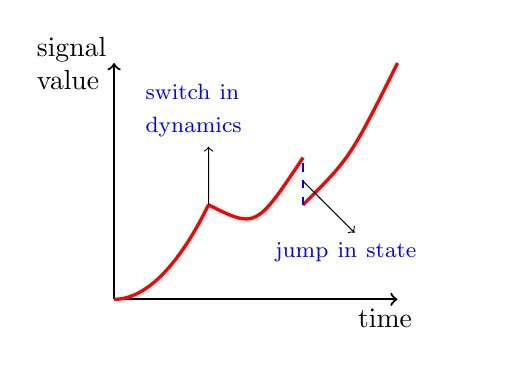
\begin{tikzpicture}[scale = 0.6]
% Create axis
\draw[thick,->] (0,0) -- (0,5);
\draw[thick,->] (0,0) -- (6,0);

% Label axis
\node[text width = 1 cm] at (-0.8,5) {signal value};
\node[text width = 1 cm] at (6,-0.4) {time};

% Create curve 1 from t=0 to t=2
\draw[red,very thick] (0,0) parabola (2,2);
% Create curve 1 from t=2 to t=4
\draw[red,very thick] (2,2) .. controls (3,1.5) .. (4,3);
% Create curve 1 from t=4 to t=6
\draw[red,very thick] (4,2) .. controls (5,3) .. (6,5);

% Label behavior of curves

% Label switch in dynamics
\node[text width = 1.6cm, blue] at (2,4)  (switch) {{\footnotesize switch in\\ dynamics}};
\draw[ ->] (2,2) -- (switch);


% Label jump in state
\node[text width = 2.5cm, blue] at (5.5,1) (jump) {{\footnotesize jump in state}};
\draw[blue, dashed] (4,2) -- (4,3);
\draw[->] (4,2.5) -- (jump);

\end{tikzpicture}
%
\end{minipage}
\begin{minipage}{0.45\textwidth}
%% Dynamics of hybrid system
%
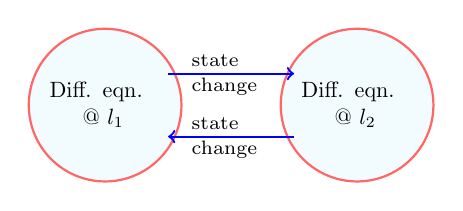
\begin{tikzpicture}[scale =0.8,
location/.style = {circle, draw=red!60, thick, fill = cyan!5}, 
]


% Draw locations
\node[text width = 2 cm, scale =0.8, location] at (0,0) {{ Diff. eqn.\\ \hspace{1.5em} @ $l_1$}};
\node[text width = 2 cm, scale =0.8, location] at (4,0) {{ Diff. eqn.\\  \hspace{1.5em} @ $l_2$}};

% Draw edges
\draw[thick, blue, ->] (1,0.5) --  (3,0.5);
\draw[thick, blue, <-] (1,-0.5) --  (3,-0.5);

% Label edges
\node[text width = 1cm] at (2,0.7) {\scriptsize state};
\node[text width = 1cm] at (2,0.3) {\scriptsize change};
\node[text width = 1cm] at (2,-0.3) {\scriptsize state};
\node[text width = 1cm] at (2,-0.7) {\scriptsize change};

\end{tikzpicture}\\[0.5em]
%
$x\in\reals^n$: Continuous state.\\
$l\in\set{l_1,...,l_k}$: Discrete state.
\end{minipage}

\begin{minipage}{0.45\textwidth}
\begin{figure}
\center
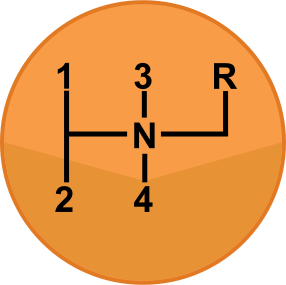
\includegraphics[width = 3cm, height = 3cm]{figures/downloaded/CarGear.png}
\caption{\small Gear control to switch dynamics}
\end{figure}
\end{minipage}
%
\begin{minipage}{0.45\textwidth}
\begin{figure}
\includegraphics[height = 3cm, width = 2.5cm]{figures/downloaded/ComputerControl.jpg}
\caption{\small Computer Control System}
\end{figure}
\end{minipage}

\end{frame}


%=========================================================================================================================================

\begin{frame}{Verification of Hybrid Systems is Challenging}
%
\begin{itemize}
\item For most hybrid system, computing set of reachable states is \negemph{ undecidable} or \negemph{ computationally expensive}.
{\bf TODO give references}
\item Consider a simple \negemph{ discrete time affine switched system}:
\[
x(t+1) = A_ix(t)+u_i,~~i\in\set{1,2}.
\]
%
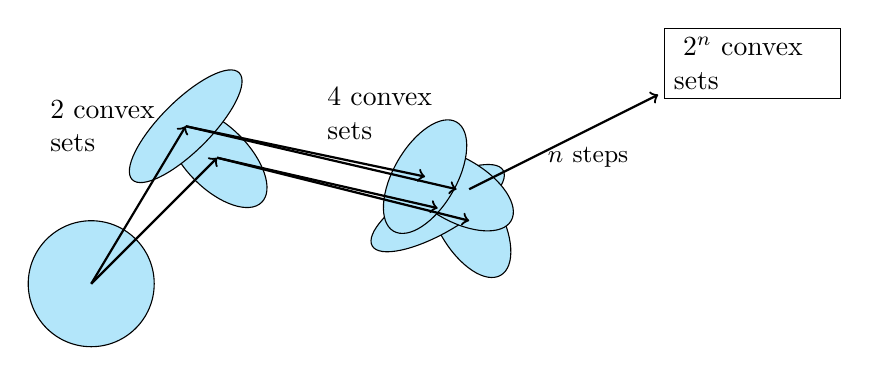
\begin{tikzpicture}[scale = 0.8
]
\draw[fill=cyan!30] (0,0) circle (1cm);

\draw[rotate around = {45:(2,2)}, fill=cyan!30] (2,2) ellipse (0.5cm and 1cm);
\draw[rotate around = {135:(1.5,2.5)}, fill=cyan!30] (1.5,2.5) ellipse (0.4cm and 1.2cm);
\draw[->,thick] (0,0) -- (2,2);
\draw[->,thick] (0,0) -- (1.5,2.5);
\node[text width = 2cm] at (0.6, 2.5) {$2$ convex sets};

\draw[rotate around = {30:(6,1)}, fill=cyan!30] (6,1) ellipse (0.5cm and 1cm);
\draw[rotate around = {120:(5.5,1.2)}, fill=cyan!30] (5.5,1.2) ellipse (0.4cm and 1.2cm);
\draw[rotate around = {60:(5.8,1.5)}, fill=cyan!30] (5.8,1.5) ellipse (0.5cm and 1cm);
\draw[rotate around = {150:(5.3,1.7)}, fill=cyan!30] (5.3,1.7) ellipse (0.5cm and 1cm);
\draw[->,thick] (2,2) -- (6,1);
\draw[->,thick] (2,2) -- (5.5,1.2);
\draw[->,thick] (1.5,2.5) -- (5.3,1.7);
\draw[->,thick] (1.5,2.5) -- (5.8,1.5);
\node[text width = 2cm] at (5, 2.7) {$4$ convex sets};

\draw[->,thick] (6,1.5) -- (9,3);
\node[text width = 2cm] at (8.5,2) {\small $n$ steps};
\node[draw,text  width = 2cm]  at (10.5,3.5) {\negemph{ $2^n$ convex\\ sets}};
\end{tikzpicture}
%
\end{itemize}
%
\end{frame}

%==========================================================================================================================

\begin{frame}{Over-approximation Using Set Representation}
To deal with \negemph{ undecidability} or \negemph{ high computational complexity} of representing reachable sets:
%
\begin{itemize}
\item \posemph{Over-approximate} them by a \posemph{ set} which can be \posemph{ encoded} and \posemph{ manipulated efficiently}.
\item use \plemph{ Set Representation}:  A \posemph{ digital encoding} of a possibly infinite \posemph{ set of states}.
\end{itemize}
%

\begin{minipage}{0.35\textwidth}
% Polytopic approximation of reachable set
\center{
\begin{tikzpicture}[scale=0.9]
\draw[rotate around = {30:(6,1)}, fill=cyan!30] (6,1) ellipse (0.5cm and 1cm);
\draw[rotate around = {120:(5.5,1.2)}, fill=cyan!30] (5.5,1.2) ellipse (0.4cm and 1.2cm);
\draw[rotate around = {60:(5.8,1.5)}, fill=cyan!30] (5.8,1.5) ellipse (0.5cm and 1cm);
\draw[rotate around = {150:(5.3,1.7)}, fill=cyan!30] (5.3,1.7) ellipse (0.5cm and 1cm);
% draw lines of polytope around above image
\draw[very thick,color=onyx] (4.38,0.53)--(5,2.7);
\draw[very thick,color=onyx] (5,2.7)--(5.8,2.6);
\draw[very thick,color=onyx] (5.8,2.6)--(6.6,1.75);
\draw[very thick,color=onyx] (6.6,1.75)--(6.8,0.9);
\draw[very thick,color=onyx] (6.8,0.9)--(6.575,0);
\draw[very thick,color=onyx] (6.575,0)--(4.38,0.53);
\end{tikzpicture}
}
%
\begin{exampleblock}{Polytopes}
\eqnemph{$\set{x:Tx\leq d, x\in\reals^n}$}\\
{\small $T\in\mat{m}{n}{\reals}$, ${d\in\reals^m}$.}
\end{exampleblock}
%
\end{minipage}
%
\hspace{2.5em}
\begin{minipage}{0.4\textwidth}
%
\vspace{-0.5em}
\centering{
%
\begin{tikzpicture}[scale=0.8]x
\draw[rotate around = {30:(6,1)}, fill=cyan!30] (6,1) ellipse (0.5cm and 1cm);
\draw[rotate around = {120:(5.5,1.2)}, fill=cyan!30] (5.5,1.2) ellipse (0.4cm and 1.2cm);
\draw[rotate around = {60:(5.8,1.5)}, fill=cyan!30] (5.8,1.5) ellipse (0.5cm and 1cm);
\draw[rotate around = {150:(5.3,1.7)}, fill=cyan!30] (5.3,1.7) ellipse (0.5cm and 1cm);
% draw ellipse around the above image
\draw[color=onyx, very thick, rotate around={70:(5.7,1.1)}] (5.7,1.1) ellipse (1.65cm and 1.225cm);
\end{tikzpicture}
%
}
%
\hspace{0.5em}
\begin{exampleblock}{Ellipsoid}
\eqnemph{$\set{x: x^TPx\leq 1, x\in\reals^n}$}.\\
{\small $P\in\mat{n}{n}{\reals}$: Positive semi-definite.}
\end{exampleblock}
%
\end{minipage}
%
\end{frame}

%====================================================================================================================================

\begin{frame}{Positive Invariant for Unbounded Time
Over-approximation}
Typically use \plemph{Positive Invariant} (PI) to approximate reachable
set for \posemph{unbounded/all time/s}.
%
\begin{block}{}
$\Psi: Positive Invariant\implies \forall x\in\Psi, \operatorname*{Next}(x)\in\Psi$.
\end{block}
%
\hspace{1.5em}
\begin{minipage}{0.45\textwidth}
\eqnemph{
({\small {Initial~Set}$\subseteq$ PI)$\implies$ \\(Unbounded(t) 
reach set $\subseteq$ PI).}
}
\end{minipage}
%
\begin{minipage}{0.35\textwidth}
\center{
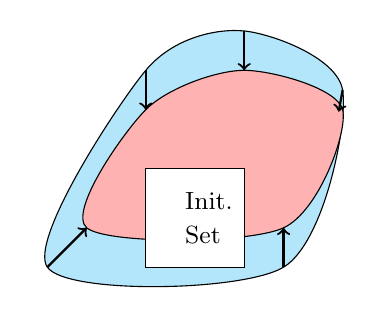
\begin{tikzpicture}[scale=2.5]
\draw[fill=cyan!30] plot[smooth cycle] coordinates {(0,0) (0.5,1)
(1,1.2) (1.5,0.9) (1.2,0) };
\draw[fill=red!30] plot[smooth cycle] coordinates {(0.2,0.2) (0.5,0.8)
(1,1) (1.5,0.8) (1.2,0.2) };
\draw[->,thick] (0,0)--(0.2,0.2);
\draw[->,thick] (0.5,1)--(0.5,0.8);
\draw[->,thick] (1,1.2)--(1,1);
\draw[->,thick] (1.5,0.9) -- (1.48,0.79);
\draw[->,thick] (1.2,0)--(1.2,0.2);
\draw[fill=white] (0.5,0) rectangle (1,0.5);
\node[text width = 0.25cm] at (0.75, 0.25) {\small Init.\\ Set };
\end{tikzpicture}
}
\end{minipage}
%
\end{frame}

%=====================================================================================================================================

\begin{frame}{Desirable Features of a Set Representation}
\begin{itemize}
\item \posemph{Accurate} and \posemph{fast computation} of  reachable states $\Leftarrow$
\begin{enumerate}
\item \plemph{Closure} under set operations involved in computing reachable sets.
\item \plemph{Low computational complexity} of set operations involved in computing reachable sets.
\item \plemph{Existence} and \plemph{efficient encoding} of \plemph{positive invariants} for \plemph{stable linear transformations}.
\end{enumerate}
\end{itemize}
\pause
%
For \posemph{affine hybrid systems}, like \eqnemph{
%
\begin{align*}
& \text{if}~T_{\trj{l}{t}}\trj{x}{t}\leq 1,~~ \trj{l}{t+1}=f(\trj{l}{t})\\
& \trj{x}{t+1}=
A_{\trj{l}{t}}\trj{x}{t}+\trj{u}{t}.
\end{align*}
}
%
Set operations typically used in reachability computations:\\
\plemph{Linear transformation}, \plemph{Minkowski sum}, \plemph{Intersection with half-spaces}.
\end{frame}

%=======================================================================================================================================

\begin{frame}{Features of Polytopes and Ellipsoids}
%
\begin{minipage}{0.48\textwidth}
\underline{\plemph{Polytope}}:
\begin{enumerate}
\item \emph{Linear transformation}: \posemph{Efficient} for \posemph{invertible matrix};
\negemph{Otherwise Exponential Complexity}.
\item \emph{Minkowski sum}: More than \negemph{Exponential
Complexity}.
\item \emph{Positive Invariant}: \posemph{Exists} for stable linear
transformation, but \negemph{compleixty of encoding} is \negemph{unbounded}.
\end{enumerate}
\end{minipage}
%
\begin{minipage}{0.48\textwidth}
\underline{\plemph{Ellipsoid}}:
%
\begin{enumerate}
\item \emph{Invertible Linear transformation} is \posemph{efficiently
computable}.
\item \emph{Minkowski sum}: \negemph{Not closed}.
\item \emph{Positive Invariant}: \posemph{Exists}
and \posemph{Efficiently encodable} for stable linear transformation.
\end{enumerate}
%
\end{minipage}
%
\end{frame}

%==================================================================================================================================

\begin{frame}{Simple Zonotope}
A \plemph{zonotope} is a \plemph{projection} of \plemph{higher dimensional hypercube}
onto \plemph{lower dimensional} space.\\[0.5em]
%
Let  \emph{ $V\in\mat{n}{m}{\reals}$: Generator matrix},
 \emph{$c\in\reals^n$: center}.
 %
\begin{block}{}
\center{
\eqnemph{
$
\rztope{\ptemp}{\cen}:=\set{\cen+\ptemp\zeta:~\zeta\in[-1,1]^m}.
$
}
}
%
\end{block}
%
\vspace{0.5em}
%
\begin{minipage}{0.43\textwidth}
{\scriptsize $V=\mymatrix{1 &   -1 &          0 &    0.5 \\
   -1 &         0 &   -1 &    0.5}$}
\includegraphics[scale=0.25]{figures/CZtopes/RealZonotope.jpg}
\end{minipage}
%
\vline
%
\begin{minipage}{0.55\textwidth}
\begin{enumerate}
\item \posemph{Advantage} over \posemph{polytope} for linear transformation.
%
\eqnemph{\[
A\rztope{\ptemp}{\cen}=\rztope{A\ptemp}{A\cen}.
\]}
%
\vspace{-2em}
\item \posemph{Advantage} over \posemph{ellipsoid} and \posemph{polytope} for Minkowski sum.
%
\eqnemph{\begin{align*}
& \rztope{\ptemp}{\cen}\oplus\rztope{\ptemp^\pr}{\cen^\pr}\\
& = \rztope{\mymatrix{\ptemp & \ptemp^\pr}}{\cen+\cen^\pr}.  
\end{align*}}
%
\end{enumerate}
%
\end{minipage}
%
\end{frame}

%==================================================================================================================================


\begin{frame}{Drawback of Zonotopes for Computing Positive Invariants}
\begin{itemize}
\item \negemph{Directions for convergence} to an \negemph{equilibrium} can be
encoded by \negemph{complex valued eigenvectors}.
\item Usual \negemph{zonotopes} only have
\negemph{real eigenvectors} as \negemph{generators}.
\end{itemize}
%
\pause
%
\begin{block}{}
{\small
Let \emph{$A\in\mat{n}{n}{\reals}$} has \emph{$\mu\in[-1,1]^n$: real
eigenvalues} and \emph{$\ptemp\in\mat{n}{n}{\reals}$: eigenvectors} as
\emph{column vectors}, i.e., \emph{$A\ptemp = \ptemp\diagonal{\mu}$}.
}
\eqnemph{\[
A\lt(\rztope{\ptemp}{0}\rt)\subseteq \rztope{\ptemp}{0}
\]}
\vspace{-1em}
\end{block}
%
\negemph{*} We \negemph{can not rely} on above proposition when \negemph{eigenvectors are complex}.
\end{frame}

%==================================================================================================================================

\begin{frame}{Complex Zonotope: A New Set Representation}

{\small
\begin{itemize}
\item Extend \posemph{simple zonotope to complex numbers} in a way that can \posemph{capture
contraction along complex vectors}.
\item \plemph{Complex valued generators} with \plemph{Complex combining
coefficients} whose \plemph{absolute value $<=1$}.
\item Geometrically, \plemph{Minkowski sum} of \plemph{Ellipses}
and \plemph{Line Segments}.
\end{itemize}
%
$\ptemp\in\mat{n}{m}{\compnums}$, $\cen\in\reals^n$.
}
%
\begin{block}{}
\center{
\eqnemph{$
\cztope{\ptemp}{\cen} := \set{\ptemp\zeta+\cen:~\zeta\in\compnums^m,~\infnorm{\zeta}\leq 1}.
$}
}
\end{block}
%
\begin{minipage}{0.35\textwidth}
%
\begin{tikzpicture}[scale=1]
\node[text width = 1cm] at (0,2) {{\small $\mymatrix{1+2\iota\\1-2\iota}$}};
\draw[thick,fill=cyan!30, rotate around = {135:(0,0)}] (0,0) ellipse
(1cm and 0.5cm);
\draw[->] (0,1.5)--(0,0.8);
\node at (1.5,1){$\bigoplus$};
\end{tikzpicture}
%
\end{minipage}
%
\begin{minipage}{0.3\textwidth}
%
\begin{tikzpicture}[scale=0.8]
\node[text width = 1cm] at (0,3.5) {{\small $\mymatrix{1\\1}$}};
\draw[color=blue,very thick] (-0.5,0.5)--(1,2);
\draw[->] (-0.2,3)--(-0.2,1.5);
\node at (1.5,2.5){$\bigoplus$};
\end{tikzpicture}
%
\end{minipage}
%
\begin{minipage}{0.3\textwidth}
%
\begin{tikzpicture}[scale=1]
\node[text width = 1cm] at (0,2) {{\small$\mymatrix{2+\iota\\2-\iota}$}};
\draw[thick,fill=cyan!30, rotate around = {45:(0,0)}] (0,0) ellipse
(1cm and 0.5cm);
\draw[->] (0,1.5)--(0,0.8);
\end{tikzpicture}
%
\end{minipage}
%
\end{frame}

%==================================================================================================================================

\begin{frame}{Non-polytopic Projection of Complex Zonotope}
%
\begin{figure}
\center
\includegraphics[scale=0.3]{figures/CZtopes/xycz.png}
\includegraphics[scale=0.3]{figures/CZtopes/yzcz.png}\\
\includegraphics[scale=0.3]{figures/CZtopes/xzcz.png}
%\caption{Real projection of complex zonotope on axis oriented hyperplanes}~\label{fig:3dcztope}
\end{figure}
%
\end{frame}

%==================================================================================================================================

\begin{frame}{Contraction Along Complex Eigenvectors}

\begin{block}{}
{\small
Let \plemph{$A\ptemp = \ptemp\diagonal{\mu}$}:
$\ptemp\in\mat{n}{n}{\compnums}$ and $\mu\in\compnums^n$.
}

\begin{enumerate}
\eqnemph{
\item $A\lt(\cztope{\ptemp}{0}\rt)
= \cztope{\ptemp\diagonal{{\mu}}}{0}.$
\item If
$\infnorm{\mu}\leq 1$, then
$A\lt(\rztope{\ptemp}{0}\rt)\subseteq \rztope{\ptemp}{0}$.
}
\end{enumerate}
%
\end{block}
%
\begin{figure}
\center
\includegraphics[scale=0.25]{figures/CZtopes/eigcontraction.png}\\
\includegraphics[scale=0.25]{figures/CZtopes/contraction-zonotope.png}
%\caption{Contraction of complex zonotope along
%eigenvectors}~\label{fig:cz-scaled-down}
\end{figure}
%
\end{frame}

\begin{frame}{Problem with Refining a Complex Zonotope}
\negemph{*} \negemph{Better approximation} by complex
zonotope \negemph{can not} be found by \negemph{adding generator}.
%
\begin{enumerate}
\item \negemph{Increases size}.
\item \negemph{Distorts positive invariance}.
\end{enumerate}
%
\begin{figure}
\center
\includegraphics[scale=0.3]{figures/CZtopes/refinement.png}
%% \caption{Violation of positive invariance and size increase after
%% adding a generator to the basic representation.}~\label{fig:refinement}
\end{figure}
%
\end{frame}
%
\begin{frame}{Template Complex Zonotope}
\plemph{Variable bounds} on absolute values of \plemph{combining
coefficients}.\\[0.5em]

{\small
${\ptemp\in\mat{n}{m}{\compnums}}$: \plemph{template},
\fbox{${\sfact\in\reals^m_{\geq 0}}$: \plemph{scaling factors}},
${\cen\in\reals^n}$: \plemph{center}.
}
%
\begin{block}{}
%
\center{\eqnemph{
$
\tcztope{\ptemp}{\cen}{\sfact}
= \set{\ptemp\zeta+\cen:~\absolute{\zeta_i}\leq \sfact_i~\forall
i\in\set{1,...,m}}.
$
}}
\end{block}
%
\begin{itemize}
\item \posemph{Add more generators} and \posemph{adjust scaling} factors to find \posemph{better approximations}.
\end{itemize}
%
[TODO: ADD FIGURE HERE]\\
Similar to \posemph{template polyhedron}~{TODO: CITE REFERENCES}.
\end{frame}
%
\begin{frame}{Basic Operations: Template Complex Zonotope}
%
\begin{enumerate}
\eqnemph{
\item
$A\tcztope{\ptemp}{\cen}{\sfact}=\tcztope{A\ptemp}{A\cen}{\sfact}$.
\item $\minsum{\tcztope{\ptemp}{\cen}{\sfact}}{\tcztope{\ptemp^\pr}{\cen^\pr}{\sfact^\pr}}
= \tcztope{\begin{bmatrix}\ptemp
& \ptemp^\pr\end{bmatrix}}{\cen+\cen^\pr}{\begin{bmatrix}\sfact\\\sfact^\pr\end{bmatrix}}$.
}
\item {\small Let $\supp{v}{\Psi}=\sup_{x\in\Psi}v^Tx$}. Then \plemph{support
function}\\
\eqnemph{
\[
\supp{v}{\real\lt(\tcztope{\ptemp}{\cen}{\sfact}\rt)}=v^Tc+\absolute{v^T\ptemp}\sfact.
\]
}
\end{enumerate}
%
\begin{itemize}
\item Above are \posemph{affine functions} of \posemph{center}
and \posemph{scaling factors}.
\end{itemize}
%
\end{frame}
%
\begin{frame}{Checking Inclusion}
Generally, checking inclusion between complex zonotopes requires \negemph{non-convex
optimization}.
But we propose a \posemph{convex relaxation} that  \posemph{works well
in practice}.\\[0.5em]
%
{\small 
%
\begin{definition}[\eqnemph{$\tcztope{\ptemp^\pr}{\cen^\pr}{\sfact^\pr}\order\tcztope{\ptemp}{\cen}{\sfact}$}]
%
\vspace{-1em}
\begin{align*}
& \exists \tmat\in\mat{m}{r}{\compnums},\tvect\in\compnums^m~~\text{such
that}\\
& \ptemp\tmat=\ptemp^\pr\diagonal{\sfact^\pr},~~\ptemp\tvect=\cen^\pr-\cen~\\%\numberthis\label{eqn:inclusion-tcz1}\\
& \max_{i=1}^m\lt(\absolute{\tvect_i}+\sum_{j=1}^r\absolute{\tmat_{ij}}-\sfact_i\rt)\leq
0.
\end{align*}
%
\end{definition}
}
\vspace{0.3em}
\begin{minipage}{0.37\textwidth}
\begin{exampleblock}{}
\center{\eqnemph{Result: 
$\order\implies\subseteq$.
}}
\end{exampleblock}
\end{minipage}
%
\begin{minipage}{0.6\textwidth}
\begin{itemize}
\item $\order$: \plemph{Second order conic constraints} (convex
constraints) on \plemph{center} and \plemph{scaling factors}.
\end{itemize}
\end{minipage}
%
\end{frame}
%
\bibliographystyle{plain}
\bibliography{ref}



\end{document}

